\documentclass[12pt,a4paper]{article}
\usepackage[utf8]{inputenc}
\usepackage{amsmath,amssymb,amsfonts,amsthm}
\usepackage{geometry}
\usepackage{enumerate}
\usepackage{fancyhdr}
\usepackage{lastpage}
\usepackage{graphicx}

% Page layout
\geometry{margin=1in}
\pagestyle{fancy}
\fancyhf{}
\lhead{Lucas Cassin Cruz Burke}
\rhead{AMATH 563}
\rfoot{Page \thepage\ of \pageref{LastPage}}

% Theorem environments
\theoremstyle{definition}
\newtheorem{problem}{Problem}
\theoremstyle{remark}
\newtheorem*{solution}{Solution}

\title{AMATH 563 Homework 3}
\author{Lucas Cassin Cruz Burke}
\date{May 12, 2023}

\begin{document}

\maketitle

\section{Theory}

% Problem 1
\begin{problem}
    Let $(\mathcal H, ||\cdot||, \langle \cdot, \cdot \rangle)$ be an RKHS of functions from a set $\mathcal X \rightarrow \mathbb R$, with kernel $K$. Given a pointset $X = \{x_1, \dots, x_m \} \subset \mathcal X$ consider the interpolation problem 

    $$\begin{cases}
        \operatorname{minimize}_{u \in \mathcal H} & ||u|| \\
        \text{subject to} & u(X) = \mathbf y.
    \end{cases}$$

    Suppose the $x_m$ are distinct and that $K(X,X)$ is invertible. Prove that the minimizer $u^*$ is given by the formula

    \begin{align}
        u^* = K(\cdot, X)K(X,X)^{-1}\mathbf y.
    \end{align}
\end{problem}
\begin{solution}
    If a minimizer $u^*$ exists, then by the representer theorem it must admit a representation of the form $$u^*(\cdot) = \sum_{i=1}^m \alpha_i K(\cdot, x_i) = K(\cdot, X)\boldsymbol \alpha$$

    Additionally, to satisfy the interpolation problem we must have $u^*(X) = \mathbf y$, which means that 

    $$u^*(X) = K(X,X)\boldsymbol \alpha = \mathbf y$$

    Since we have supposed that $K(X,X)$ is invertible by our problem setup, we can invert it to solve for the representation coefficients $\boldsymbol \alpha$, giving us 

    $$\boldsymbol \alpha = K(X,X)^{-1} \mathbf y$$

    Plugging this back into our above expression for $u^*(\cdot)$ gives us equation (1):

    $$u^*(\cdot) = K(\cdot, X) K(X,X)^{-1} \mathbf y$$
\end{solution}


% Problem 2
\begin{problem}
    Let $(\mathcal H, ||\cdot||, \langle \cdot, \cdot \rangle)$ be an RKHS of functions from a set $\mathcal X \rightarrow \mathbb R$, with kernel $K$. 

\begin{enumerate}[(a)]
    % 2.A
    \item Let $\phi \in \mathcal H^*$ be a bounded linear functional on $\mathcal H$. Show that the function $K \phi : x \mapsto \phi(K(\cdot, x))$ is the Riesz representer of $\phi$ with respect to the RKHS inner product. That is, 
    \begin{align}
        \phi(f) = \langle K\phi, f \rangle.
    \end{align}

    \begin{solution}
        Let us first show that $K\phi \in \mathcal H$. For any fixed $x \in \mathcal X$ we have $K(\cdot, x): \mathcal X \rightarrow \mathbb R$. Additionally, since $\mathcal H$ is an RKHS its kernel $K$ must be bounded and continuous, from which it follows that $K(\cdot, x) \in \mathcal H$. Since $\phi \in \mathcal H^*$ is bounded and continuous linear functional on $\mathcal H$ it follows that $(K\phi)(x) = \phi(K(\cdot, x)) \in \mathbb R$. Additionally, since $\phi$ and $K(\cdot, x)$ are each bounded, the function $\phi(K(\cdot, x))$ must also be bounded, which implies that $K\phi \in \mathcal H$. 

        Having shown that $K\phi$ is a member of $\mathcal H$, we must show that it is the Riesz representer of $\phi$ with respect to the inner product $\langle \cdot, \cdot \rangle$. Let $f \in \mathcal H$, then by the definition of $K \phi$ we write 

        $$\langle K\phi, f \rangle = \langle \phi(K(\cdot, x)), f(x) \rangle$$

        Next we may use the linearity of $\phi$ and the inner product to move $\phi$ outside of the brackets

        \begin{align*}
            \langle K\phi, f \rangle &= \langle \phi(K(\cdot, x)), f(x) \rangle \\
            &= \phi\left(\langle K(\cdot, x) , f \rangle \right)
        \end{align*}

        Lastly, we use the Riesz representation theorem to write 

        \begin{align*}
            \langle K\phi, f \rangle &= \phi\left(\langle K(\cdot, x) , f \rangle \right) \\
            &= \phi(f)
        \end{align*}

        Since $\phi(f) = \langle K\phi, f \rangle$, $K \phi$ must be the Riesz representer for $\phi$. 
    \end{solution}


    % 2.B
    \item Consider the setting of Problem 2.a. Let $\phi_1, \dots, \phi_m \in \mathcal H^*$ be a sequence of bounded linear functionals on $\mathcal H$. Show that the orthogonal complement of $\operatorname{span} \{K \phi_1, \dots, K \phi_m \}$ is precisely the subspace 
    $$\{f \in \mathcal H| \phi_j(f) = 0, \quad j = 1, \dots, m \}.$$
    \begin{solution}
        The orthogonal complement of $\operatorname{span} \{K \phi_1, \dots, K \phi_m \}$ is defined as the set of functions $f$ such that $\langle f, K\phi_j \rangle =0$ for all $j =1, \dots, m$. However in part (a) we found that $K \phi_i$ is the Riesz representer for the functional $\phi_i$. Hence by the Riesz representation theorem we have 

        $$\forall i \in \{1\dots m\}: \quad \langle f, K \phi_j \rangle = \phi_j(f) =0$$

        Therefore we conclude that the orthogonal complement of $\operatorname{span} \{K \phi_1, \dots, K \phi_m \}$ is the set 

        $$\{f \in \mathcal H \quad | \quad \forall j \in \{1, \dots, m\}: \quad \phi_j(f)=0 \}$$
    \end{solution}


    % 2.C
    \item Define the bounded linear operator 
    $$\boldsymbol \phi: \mathcal H \rightarrow \mathbb R^m, \qquad \boldsymbol \phi(f) := (\phi_1(f), \dots, \phi_m(f))^T,$$

    and consider the (generalized) interpolation problem 

    $$\begin{cases}
        \operatorname{minimize}_{u \in \mathcal H} & ||u|| \\
        \text{subject to} & \boldsymbol{\phi}(u) = \mathbf y.
    \end{cases}$$

    Consider the matrix $\Theta \in \mathbb R^{m \times m}$ with entries $\Theta_{ij} = \phi_i (K\phi_j)$. Prove that whenever $\Theta$ is invertible then the minimzer $u^*$ is given by the formula

    $$u^* = \sum_{j=1}^m \alpha_j^* K \phi_j, \qquad \text{ where } \quad \boldsymbol \alpha^* = \Theta^{-1} \mathbf y.$$

    \begin{solution}
        Our solution condition is that $\phi_i(u) = y_i$ for all $i = 1, \dots, m$. By the Riesz representation theorem we can write this as $$\langle K \phi_i, u \rangle = y_i$$

        Since our minimization problem depends only on inner products $\langle K \phi_i , u \rangle$, by the representer theorem the minimizer $u^*$ can be written in the form 

        $$u^* = \sum_{j=1}^m \alpha_j^* K \phi_j$$

        Plugging this in to our operator, we have 

        $$\phi_i(u^*) = \phi_i\left( \sum_{j=1}^m \alpha_j^* K \phi_j \right) = \sum_{j=1}^m \alpha_j^* \phi_i (K \phi_j) = \Theta \boldsymbol \alpha$$

        where $\Theta$ is as defined above. Therefore our solution condition is that 

        $$\Theta \boldsymbol{\alpha}^* = \mathbf y$$

        Hence, whenever $\Theta$ is invertible the coefficient vector $\boldsymbol \alpha^*$ is given by 
        
        $$\boldsymbol \alpha^* = \Theta^{-1} \mathbf y$$

        and the minimizer $u^*$ is given by 

        $$u^* = \sum_{j=1}^m \alpha_j^* K \phi_j$$
    \end{solution}
\end{enumerate}
\end{problem}


% Problem 3
\begin{problem}
    Let $L= D-W \in \mathbb R^{n \times n}$ be the unnormalized Laplacian and let $\tilde L = D^{-1/2}(D-W) D^{-1/2}$ be the normalized Laplacian. Show that 

    \begin{enumerate}[(a)]
        % 3.a.
        \item $(\lambda, \mathbf v)$ is an eigenpair of $\tilde L$ iff $\mathbf v = D^{1/2} \mathbf u$ where $\mathbf u$ solves the generalized eigenvalue problem $L \mathbf u = \lambda D \mathbf u$. 
        \begin{solution}
            Let us begin by showing that $\mathbf v$ is a eigenvector of $\tilde L$ with eigenvalue $\lambda$. We have

            \begin{align*}
                \tilde L \mathbf v &= \left(D^{-1/2} L D^{-1/2}\right) \left(D^{1/2} \mathbf u\right) \\
                &= D^{-1/2} L \mathbf u \\
                &= D^{-1/2} \lambda D \mathbf u \\
                &= \lambda D^{1/2} \mathbf u \\
                &= \lambda \mathbf v
            \end{align*}

            Hence $\mathbf v$ is an eigenvector of $\tilde L$ with eigenvalue $\lambda$. 

            Next, let's show that the converse is true. If $(\lambda, \mathbf v)$ is an eigenpair of $\tilde L$ then we have

            $$\tilde L \mathbf v = \lambda \mathbf v$$

            Substituting $\tilde L = D^{-1/2}L D^{-1/2}$ and $\mathbf v = D^{1/2} \mathbf u$ gives us

            \begin{align*}\left( D^{-1/2} L D^{-1/2} \right) \left( D^{1/2} \mathbf u \right) &= \lambda D^{1/2} \mathbf u \\
                D^{-1/2} L \mathbf u = \lambda D^{1/2} \mathbf u
            \end{align*}

            Then we can multiply each side on the left by $D^{1/2}$ to give us 

            $$L \mathbf u = \lambda D \mathbf u$$

            Hence, $(\lambda, \mathbf v)$ is an eigenpair of $\tilde L$ iff $\mathbf v = D^{1/2} \mathbf u$ where $\mathbf u$ solves the generalized eigenvalue problem $L \mathbf u = \lambda D \mathbf u$. 
        \end{solution}

        % 3.b.
        \item Show that if $G$ is a disconnected graph without isolated vertices and with $M$-connected components then $\tilde L$ has an $M$-dimensional null-space spanned by the weighted set functions $D^{1/2} \boldsymbol 1_{G_j}$ where $\boldsymbol 1_{G_j}$ is the indicator vector of the $j$-th connected component $G_j$.
        \begin{solution}
            We have a graph $G$ that is disconnected with $M$ connected components, which implies that the Laplacian $L$ of the graph can be represented as a block diagonal matrix with $M$ blocks. Each of these blocks represents the Laplacian $L_j$ of the $j$-th connected component $G_j$. 
            
            Since each component $G_j$ is connected, the Laplacian $L_j$ of the $j$-th component has a one-dimensional null space spanned by the constant vector $\boldsymbol 1_{j}$, which is the indicator vector for the component $G_j$.
            
            Given that our graph $G$ is the union of the components $G_j$, i.e., $G = \cup_{j=1}^{M} G_j$, the indicator vector $\boldsymbol 1_{G_j}$ is a null vector of $L$. Moreover, since there are no isolated vertices, any null vector of $L$ must be a linear combination of the vectors $\boldsymbol 1_{G_j}$.
            
            Since the vectors $\boldsymbol 1_{G_j}$ are linearly independent and there are $M$ of them, the dimension of the null space of $L$ is $M$. Now let $\mathbf w \in \mathbb R^M$ be a null vector of $L$. By the definition of $\tilde L$, we have 

            $$L \mathbf w = D^{1/2} \tilde L D^{1/2} \mathbf w = 0$$

            Multiplying on the left by $D^{-1/2}$ gives us 

            $$\tilde L D^{1/2} \mathbf w = 0$$

            It follows that for any null vector $\mathbf w$ of $L$ the vector $\mathbf v = D^{1/2} \mathbf w$ is a null vector of $\tilde L$. Since the basis 
            
            We showed earlier that any null vector of $L$ can be represented as the linear combination

            $$\mathbf w = \sum_{j=1}^M \alpha_j \boldsymbol 1_{G_j}$$

            Therefore any null vector $\mathbf v$ of $\tilde L$ can be represented by 

            $$\mathbf v = D^{1/2} \left(\sum_{j=1}^M \alpha_j \boldsymbol 1_{G_j} \right) = \sum_{j=1}^M \alpha_j D^{1/2}\boldsymbol 1_{G_j}$$

            Since $D^{1/2}$ is an invertible matrix the set $\{D^{1/2} I_{G_j}\}_{j=1}^M$ is linearly independent, therefore the null space of $\tilde L$ must be $M$ dimensional and spanned by the weighted set functions $D^{1/2} \boldsymbol 1_{G_j}$. 
        \end{solution}

        % 3.c.
        \item Show that $\lambda_j \le 2$ for all $j \le n$, i.e., the eigenvalues of $\tilde L$ are uniformly bounded. Can you say the same about the eigenvalues of $L$? 
        \begin{solution}
            From the definition of the normalized Laplacian $\tilde L$ we have 

            \begin{align*}
                \tilde L &= D^{-1/2} (D-W) D^{-1/2}  \\
                &= I - D^{-1/2} W D^{-1/2}
            \end{align*}

            Note that the matrix $M=-D^{-1/2} W D^{-1/2}$ is symmetric with all non-negative entries, and hence its eigenvalues are real and non-negative. Additionally, since $\tilde L$ is a normalized Laplacian matrix its rows must sum to $1$, hence by the Perron-Frobenius theorem its eigenvalues must be less than or equal to one. Since $\tilde L = I - M$ the spectra of $\tilde L$ is shifted by 1, hence the eigenvalues of $\tilde L$ must be less than or equal to $2$, and are therefore uniformly bounded.

            This does not hold for the unnormalized Laplacian $L$, since the largest eigenvalue of $L$ can be as large as the maximum degree in the graph, which can be arbitrarily large for different graphs.
        \end{solution}
    \end{enumerate}
\end{problem}

\section{Computation}

\subsection{Introduction}
In this computational exercise, we investigate the use of the graph Laplacian operator for approximating the Laplacian differential operator on arbitrary domains. We first work within the unit box and verify that the eigenvectors of the graph Laplacian converge to those of the differential operator as the number of sample points increases. Then, we modify the domain to an L-shaped region and analyze the behavior of the eigenvectors in this new setting.

\subsection{Mathematical Background}
The graph Laplacian operator is defined as $L = D - W$, where $D$ is the degree matrix and $W$ is the weight matrix of a graph $G$. The eigenvectors of the Laplacian matrix provide information about the graph's structure. In particular, the eigenvectors corresponding to the smallest eigenvalues capture large-scale structure, while the eigenvectors corresponding to the largest eigenvalues capture small-scale structure.

To construct our weighted graph $G=\{X, W\}$ we randomly distribute $m$ points $X=\{x_1, \dots, x_m\}$ in the domain, and then define the weight matrix $W$ as 

$$w_{ij} = \kappa_\varepsilon(||\mathbf x_i - \mathbf x_j||_2)$$

where $\kappa$ is the kernel defined by
\[
\kappa_\varepsilon(t) = \begin{cases}
(\pi \varepsilon^2)^{-1} & t \le \varepsilon, \\
0 & t > \varepsilon.
\end{cases}
\]

The parameter $\varepsilon >0$ controls the local connectivity of the graph and is chosen as
\[
\varepsilon = C \frac{\log(m)^{3/4}}{m^{1/2}},
\]
with $C$ being a constant, chosen to be 1 in this exercise.

The graph Laplacian matrix can be interpreted as the discretization of the negative of the Laplace differential operator, defined in 2D as 

\[
\mathcal{L} f \mapsto -\left(\frac{\partial^2 f}{\partial x_1^2} + \frac{\partial^2 f}{\partial x_2^2}\right).
\]

To demonstrate this connection, we will show that the dominant eigenvectors of the graph Laplacian $L$ converge to eigenfunction solutions to the Neumann eigenvalue problem for the operator $\mathcal L$, which are given by 

$$\psi(\mathbf x) = \cos(n \pi x_1) \cos(k\pi x_2)$$

\subsection{Algorithmic Details}
We first constructed a graph with vertices distributed uniformly at random in the unit square $\Omega=[0,1]^2$. We computed the weighted adjacency matrix $W$ using the method outlined in the prior section, and from this, we computed the Laplacian matrix $L$. We used the scipy library's function spsl.eigsh to compute the first four eigenvectors of $L$, (corresponding to the smallest eigenvalues), which are presented in Figure 1. 

Next, we considered the Neumann eigenvalue problem for differential operator $\mathcal{L}$. We computed the vectors $\boldsymbol{\psi}_1, \dots, \boldsymbol{\psi}_4$ by taking the point values of the first four eigenfunctions $\psi(x)$ at the vertices $X$.

We then compared the subspaces spanned by ${\mathbf{q}_1, \dots, \mathbf{q}_4}$ and ${\boldsymbol{\psi}_1, \dots, \boldsymbol{\psi}_4}$, respectively, by computing the Frobenius norm of the commutator of the projectors onto these subspaces, and showing that this error tends to zero as $m$ increases. 

Finally, we use this method to approximate the spectrum of $\mathcal L$ on a non-standard domain, and visualize the eigenvectors $\mathbf{q}_7, \dots, \mathbf{q}_{10}$.

\subsection{Findings}

Scatter plots of the first four eigenvectors of the graph Laplacian in the unit box domain, alongside the values of the first four eigenfunctions $\mathbf{q}_7, \dots, \mathbf{q}_{10}$ of $\mathcal L$, are shown in Figure 1 below.

\begin{figure}[h]
    \centering
    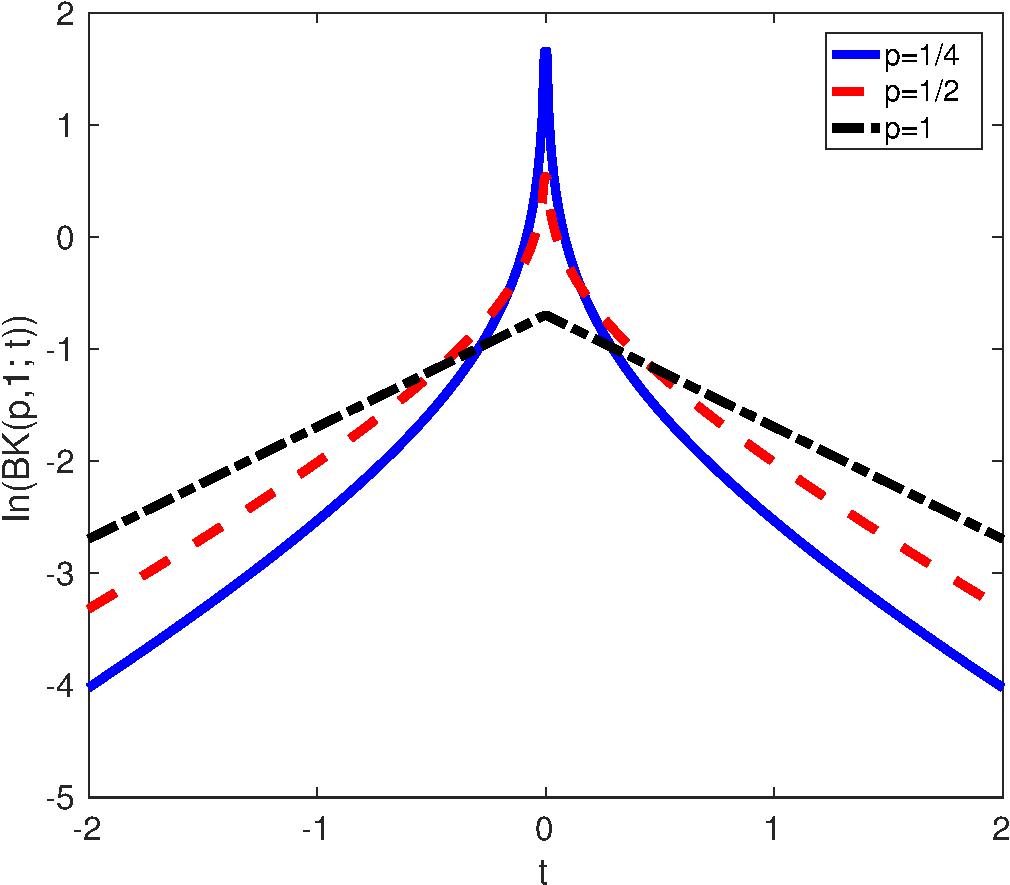
\includegraphics[width=7.5cm]{fig1.png}
    \includegraphics*[width=7.5cm]{fig2.png}
    \caption{Eigenvectors 1-4 of the graph Laplacian $L$ (left) and the alues of the four eigenfunctions of the Laplacian $\mathcal L$ (right) in the unit box.}
\end{figure}

From these images one can convince themselves that the eigenvectors in Figure 1 resemble linear combinations of the functions in Figure 2a. We verify this numerically by defining an error function as described in the prior section, shown in Figure 2a. 

\begin{figure}[h!]
    \centering
    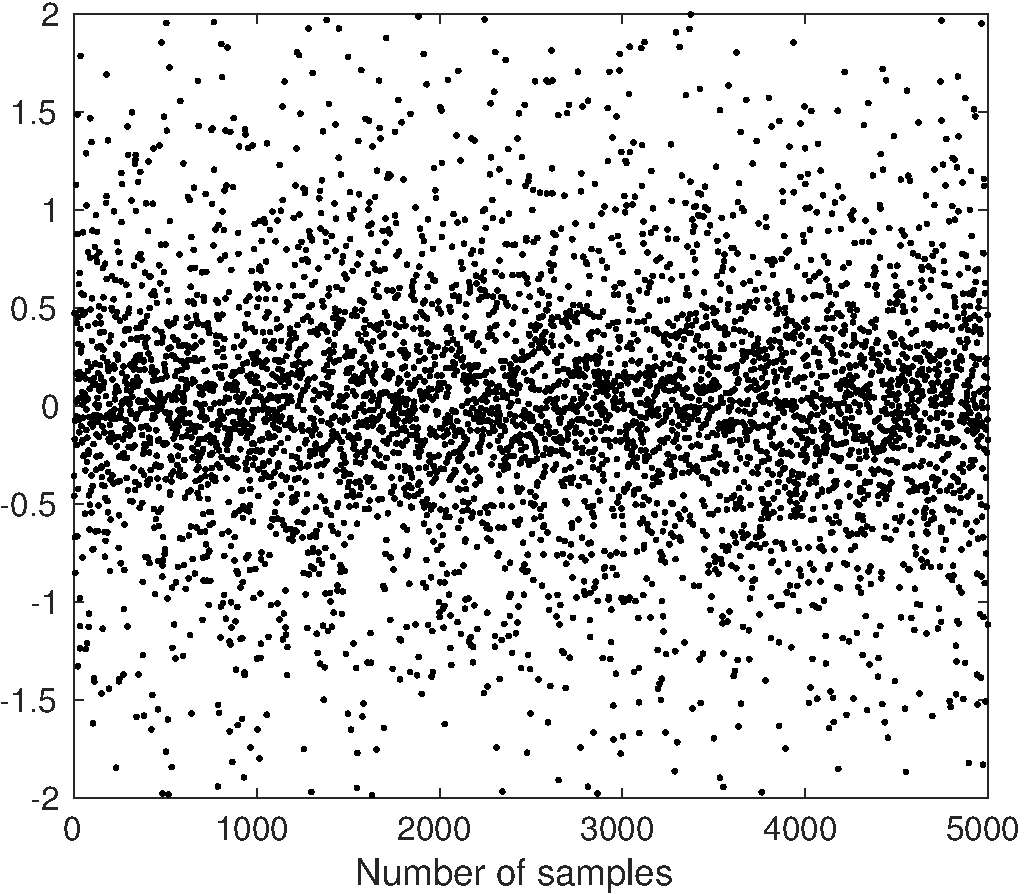
\includegraphics[width=13cm]{fig3.png}
    \includegraphics[width=13cm]{fig4.png}
    \caption{$\operatorname{error}(m)$ for $m=2^7$, $2^8$, $2^9$, $2^{10}$ between $\operatorname{span}\{\mathbf q_1, \dots, \mathbf q_4\}$ and $\operatorname{span}\{\boldsymbol{\psi}_1, \dots, \boldsymbol{\psi}_4\}$ (top), and eigenvectors 7-10 of the graph Laplacian in the L-shaped domain (bottom).}
\end{figure}

For the L-shaped domain, we compute the eigenvectors corresponding to the 7th through 10th smallest eigenvalues of the graph Laplacian and create scatter plots to visualize them. The plots are shown in Figure 2b below.


\end{document}
